\documentclass[8pt]{beamer}

\usetheme[progressbar=frametitle]{metropolis}
\usepackage{appendixnumberbeamer}

\usepackage{booktabs}
\usepackage[scale=2]{ccicons}
\usepackage{tcolorbox}
\usepackage{pgfplots}
\usepgfplotslibrary{dateplot}
\usepackage{dirtree}
\usepackage{xspace}
\newcommand{\themename}{\textbf{\textsc{metropolis}}\xspace}
\setbeamersize{text margin left=3mm,text margin right=3mm} 

\title{TrackG4PS}
\subtitle{A simulation of the CMS PS modules with cosmic rays}
% \date{\today}
\date{}
\author{Piero Viscone}
\institute{University of Pisa}
% \titlegraphic{\hfill\includegraphics[height=1.5cm]{logo.pdf}}

\begin{document}

\maketitle

\begin{frame}{Tools and libraries used}
    \begin{columns}[T,onlytextwidth]
    \column{0.5\textwidth}

    \begin{description}[align=left]
    
        \item[Geant4] Simulation toolkit
        \item[ROOT] Data analysis framework
        \item[Cmake] Makefile generator
        \item[CCache] Compiler cache
        \item[Catch2] Unit-testing
     \end{description}


    \column{0.5\textwidth}

    \begin{description}[align=parleft]
        \item[cppcheck] Static analyzer
        \item[Doxygen] Docs generator
        \item[github-actions] Docs deployment
        \item[github-pages] Docs host
        \item[cppitertools] python-like iterators
    \end{description}
\end{columns}
\vspace{0.8cm}
\begin{center}
    \textbf{Lack of CI/CD due to the size of the dependencies}.\\
    \vspace{0.15cm}
    Possible workarounds:
    \begin{itemize}
        \item Self-hosted runner: Security issues.
        \item Static linking: Not resolve the problem at all.
        \item Docker container: Exceed the guaranteed space for a free account.
    \end{itemize}
\end{center}


\end{frame}

\begin{frame}{PS modules}
       \begin{tabular}{cl}  
         \begin{tabular}{c}
          \hspace*{-8mm}
           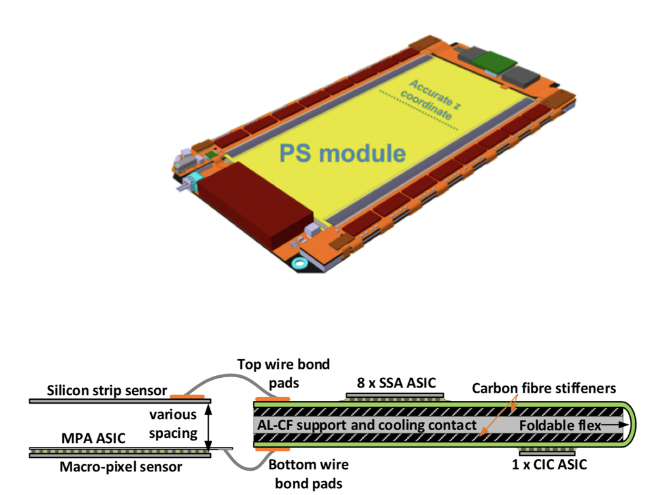
\includegraphics[height=5cm]{img/ps_module.png}
           \end{tabular}
           & \begin{tabular}{l}
           \hspace*{-6mm}
             \parbox{0.42\linewidth}{%  change the parbox width as appropiate
            PS (and 2S) modules will be the modules of the outer tracker of CMS during the Run4. 
            \newline
            \newline
            They are made of two sensors: a pixel module and a strip module. These are 300 $\mu m$ thick and spaced apart by a variable-length (1 to 4 mm).
            }
         \end{tabular}  \\
    \end{tabular}

\hspace{10cm}

\begin{columns}[T,onlytextwidth]
    \column{0.5\textwidth}
    Pixel module
    \begin{itemize}
    
        \item 960 $\times$ 32 pixel
        \item Pixel dimension $100 \mu m \; \times \; 1.5 mm$
     \end{itemize}


    \column{0.5\textwidth}
    Strips module
    \begin{itemize}
        \item 2 column of 960 strips
        \item Strip dimension $ 100 \mu m \; \times \; 2.5cm$
    \end{itemize}
\end{columns}
\end{frame}



\begin{frame}{Detector setup}
    
    

    \begin{figure}
            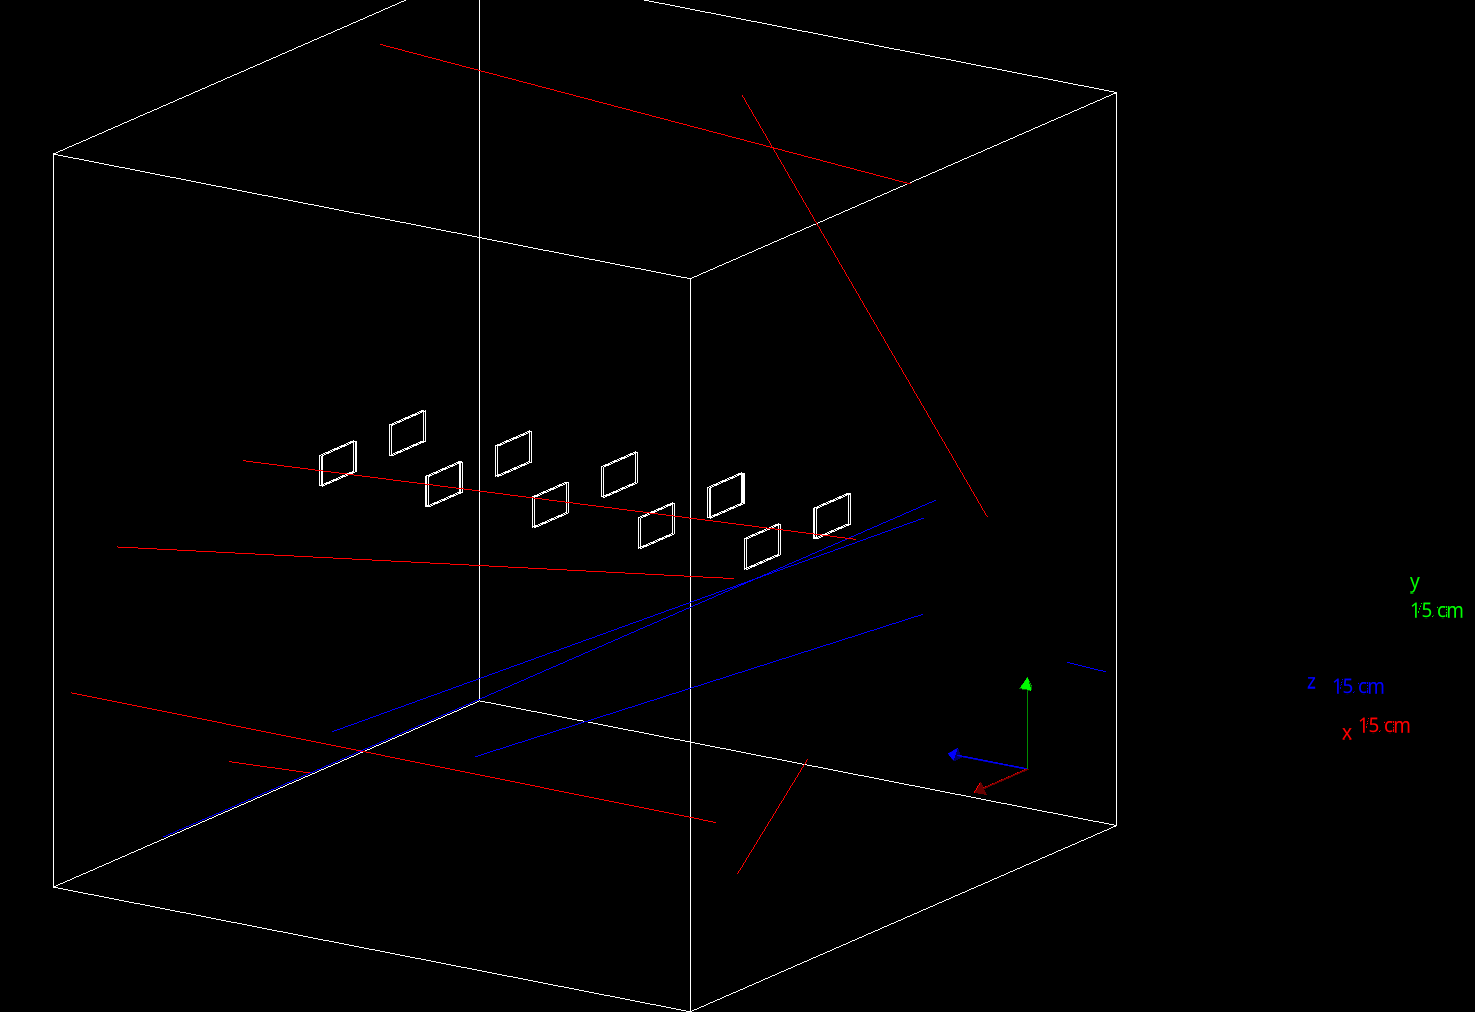
\includegraphics[height=6cm]{img/detector.png}
    \end{figure}
    These modules are currently being tested in a cryostat with cosmic rays in a grid of 2 columns and 5 layers.

    
    
    
    
                
\end{frame}

\section{Simulation}
\begin{frame}{Simulation}

   \begin{tabular}{cl}  
     \begin{tabular}{c}
      \hspace*{-8mm}
       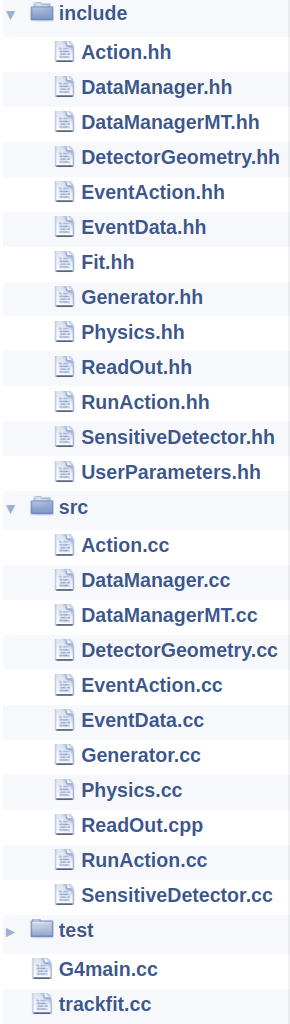
\includegraphics[height=8.5cm]{img/files.png}
       \end{tabular}
       & \begin{tabular}{p}
        \hspace{-6mm}
         \parbox{0.8\linewidth}{%  change the parbox width as appropiate
        Geant provides a lot of abstract classes.\\
        The user has to create concrete classes inheriting from these and defining their virtual methods.
        \begin{description}[align=left]
            \item[DetectorGeometry] Defines the geometry of the detector
            \item[EventAction] Defines what to do at the start/end of an event
            \item[Generator] Manage the particle gun
            \item[Physics] Defines the physical processes involved
            \item[RunAction] Defines what to do at the start/end of the run
            \item[SensitiveDetector] Defines what to do at each step in the sensitive volumes
        \end{description}
        \vspace{0.12cm}
        \hline
        \vspace{0.12cm}
        Other classes was also implemented
        \begin{description}[align=left]
            \item [ReadOut] Manage the ReadOut
            \item [EventData] The class object to fill with the data
            \item [DataManager \& DataManagerMT] Manage the output files and data
        \end{description}
        \\
          \metroset{block=fill}
            \vspace{0.25cm}
        \begin{tcolorbox}[colback=green!30]
                 All simulation parameters are grouped into namespaces in UserParameters.hh and can be changed to try different configurations.      
        \end{tcolorbox}
             


        
        }     
    \end{tabular}  \\
    \end{tabular}


\end{frame}


\begin{frame}{Physics}
The Physics module defined was \textbf{G4EMStandardPhysics}.\\
It defines:
\begin{itemize}
    \item Compton Scattering, Photoelectric effect and pair production for photons.
    \item Positron annihilation
    \item Ionization, Bremsstrahlung, and multiple scattering for $e$ and $\mu$
    \item Pair production by $\mu$
\end{itemize}
\\
\\
\vspace{1cm}
Cut in range for $e^+$, $e^-$ set to avoid the production of low energy delta rays:
\begin{itemize}
    \item 10cm in Air
    \item 0.1mm in Silicon
\end{itemize}
    
\end{frame}

\begin{frame}{Particle Gun}

The \textbf{particle gun} is generated in a random position on the face of the world box.\\
Muons generated according the cosmic rays:
\begin{itemize}
    \item Charge ratio $\mu^+/\mu^-=1.3$
    \item Angular distribution $\cos^2(\theta)$
    \item Energy distribution $\frac{dN_{\mu}}{dE_{\mu} d \Omega} \approx \frac{0.14 E_{\mu}^{-2.7}}{cm^2 \; s \;sr \; GeV} \left( \frac{1}{1+\frac{1.1 E_{\mu}\cos{\theta}}{115 GeV}} + \frac{0.054}{1+\frac{1.1 E_{\mu}\cos{\theta}}{850 GeV}} \right)$ between 1 GeV and 1 TeV
\end{itemize}
\vspace{0.6cm}
All parameters are generated at the beginning of each event with the method GetRandom of ROOT::TF1.


\end{frame}

\begin{frame}{ReadOut}
Geant provides G4VReadOutGeometry: the documentation about this class is inexistent, so a simple ReadOut class was made from scratch.\\

\vspace{1cm}
To transform the position of the hit to the position of the channel hit.
\begin{enumerate}
    \item find the position of the closest module to the hit on a given axis
    \item translates the hit position in the frame of the module
    \item calculate the position of the center of the channel that was hit in the module frame
    \item translates back to the world frame
\end{enumerate}
\vspace{0.3cm}
\begin{center}
    This is applied to the 3 axes separately.
\end{center}

\end{frame}

\begin{frame}{Trigger}
  The trigger implemented is very simple:
\begin{itemize}
    \item \textbf{Pulse height discrimination:} Rejects all hits with released energy below a given threshold (40 keV).
    \\
    The main scope of the pulse height discrimination is to limit the presence of delta rays' hits in the data.
    \item \textbf{Coincidence}: Accept only events with hits in at least two different module layers.
\end{itemize}
  
\end{frame}

\begin{frame}{DataManager}
Geant provides the class G4VAnalysisManager:
\begin{itemize}
    \item Inconvenient to manage trees
    \item Inconvenient to fill them with custom object
\end{itemize}
\textbf{Solution}: use directly \textbf{ROOT methods} and a \textbf{custom data manager} to share the ROOT objects among different classes.
\\
\vspace{0.8cm}
The \textbf{DataManager} class is a singleton that contains a TFile, a TTree, and a custom event object. \\
\vspace{0.4cm}
In this way, we can obtain the same TFile, TTree, or Event object when we need it in the virtual methods of different classes and use the ROOT methods directly to fill the tree and manage the file. 

    
\end{frame}




\begin{frame}{Event object}
The data are stored in a root file with a single branch containing a custom Event object.

   \begin{tabular}{cl}  
     \begin{tabular}{c}
      \hspace*{-8mm}
      \vspace{0.4cm}
       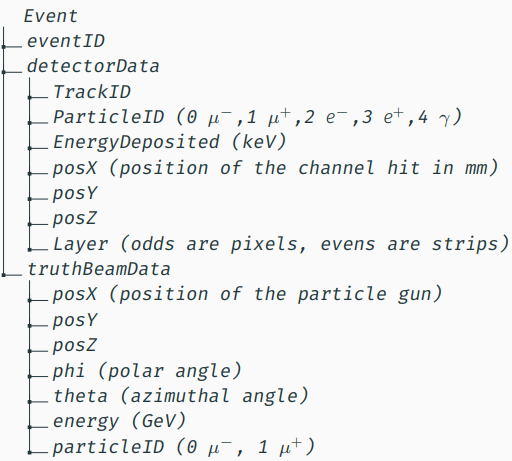
\includegraphics[height=6cm]{img/event_obj.png}
       \end{tabular}
       & \begin{tabular}{p}
        \hspace{-8mm}
         \parbox{0.45\linewidth}{%  change the parbox width as appropiate
    \begin{itemize}
        \item eventID is obtained in MyEventAction::EndOfEventAction virtual method
        \item The detector data is obtained in MySensitiveDetector::ProcessHits virtual method
        \item The beam data is obteined in MyPrimaryGenerator::GeneratePrimaries virtual method
    \end{itemize}
        }     
    \end{tabular}  \\
    \end{tabular}

\end{frame}

\begin{frame}[fragile]{Thread safety}
\textbf{Geant strategy}: Each thread works on a different file and different events.\\
\vspace{0.2cm}
\textbf{Problem}: DataManager is a singleton. All threads get the same TFile and Event object\\
\vspace{0.8cm}
The \textbf{DataManagerMT} singleton class is a friend class of DataManager.\\
\vspace{0.3cm}
It accesses the private constructor of DataManager to create multiple instances of DataManager, one each thread\\
\vspace{0.3cm}
At the beginning of the run, the master thread creates the DataManagerMT instance; then, each worker thread can obtain its own DataManager object\\
\vspace{0.6cm}
\begin{center}
    
\includegraphics[width=0.6\textwidth]{img/achievement.png}
\end{center}
\end{frame}

\begin{frame}{Results}
\begin{center}
    1819 events accepted by the trigger over 500.000 particles generated by the particle gun.\\
\end{center}

\vspace{1.5cm}

   \begin{tabular}{cl}  
     \begin{tabular}{c}
      \hspace*{-9mm}
       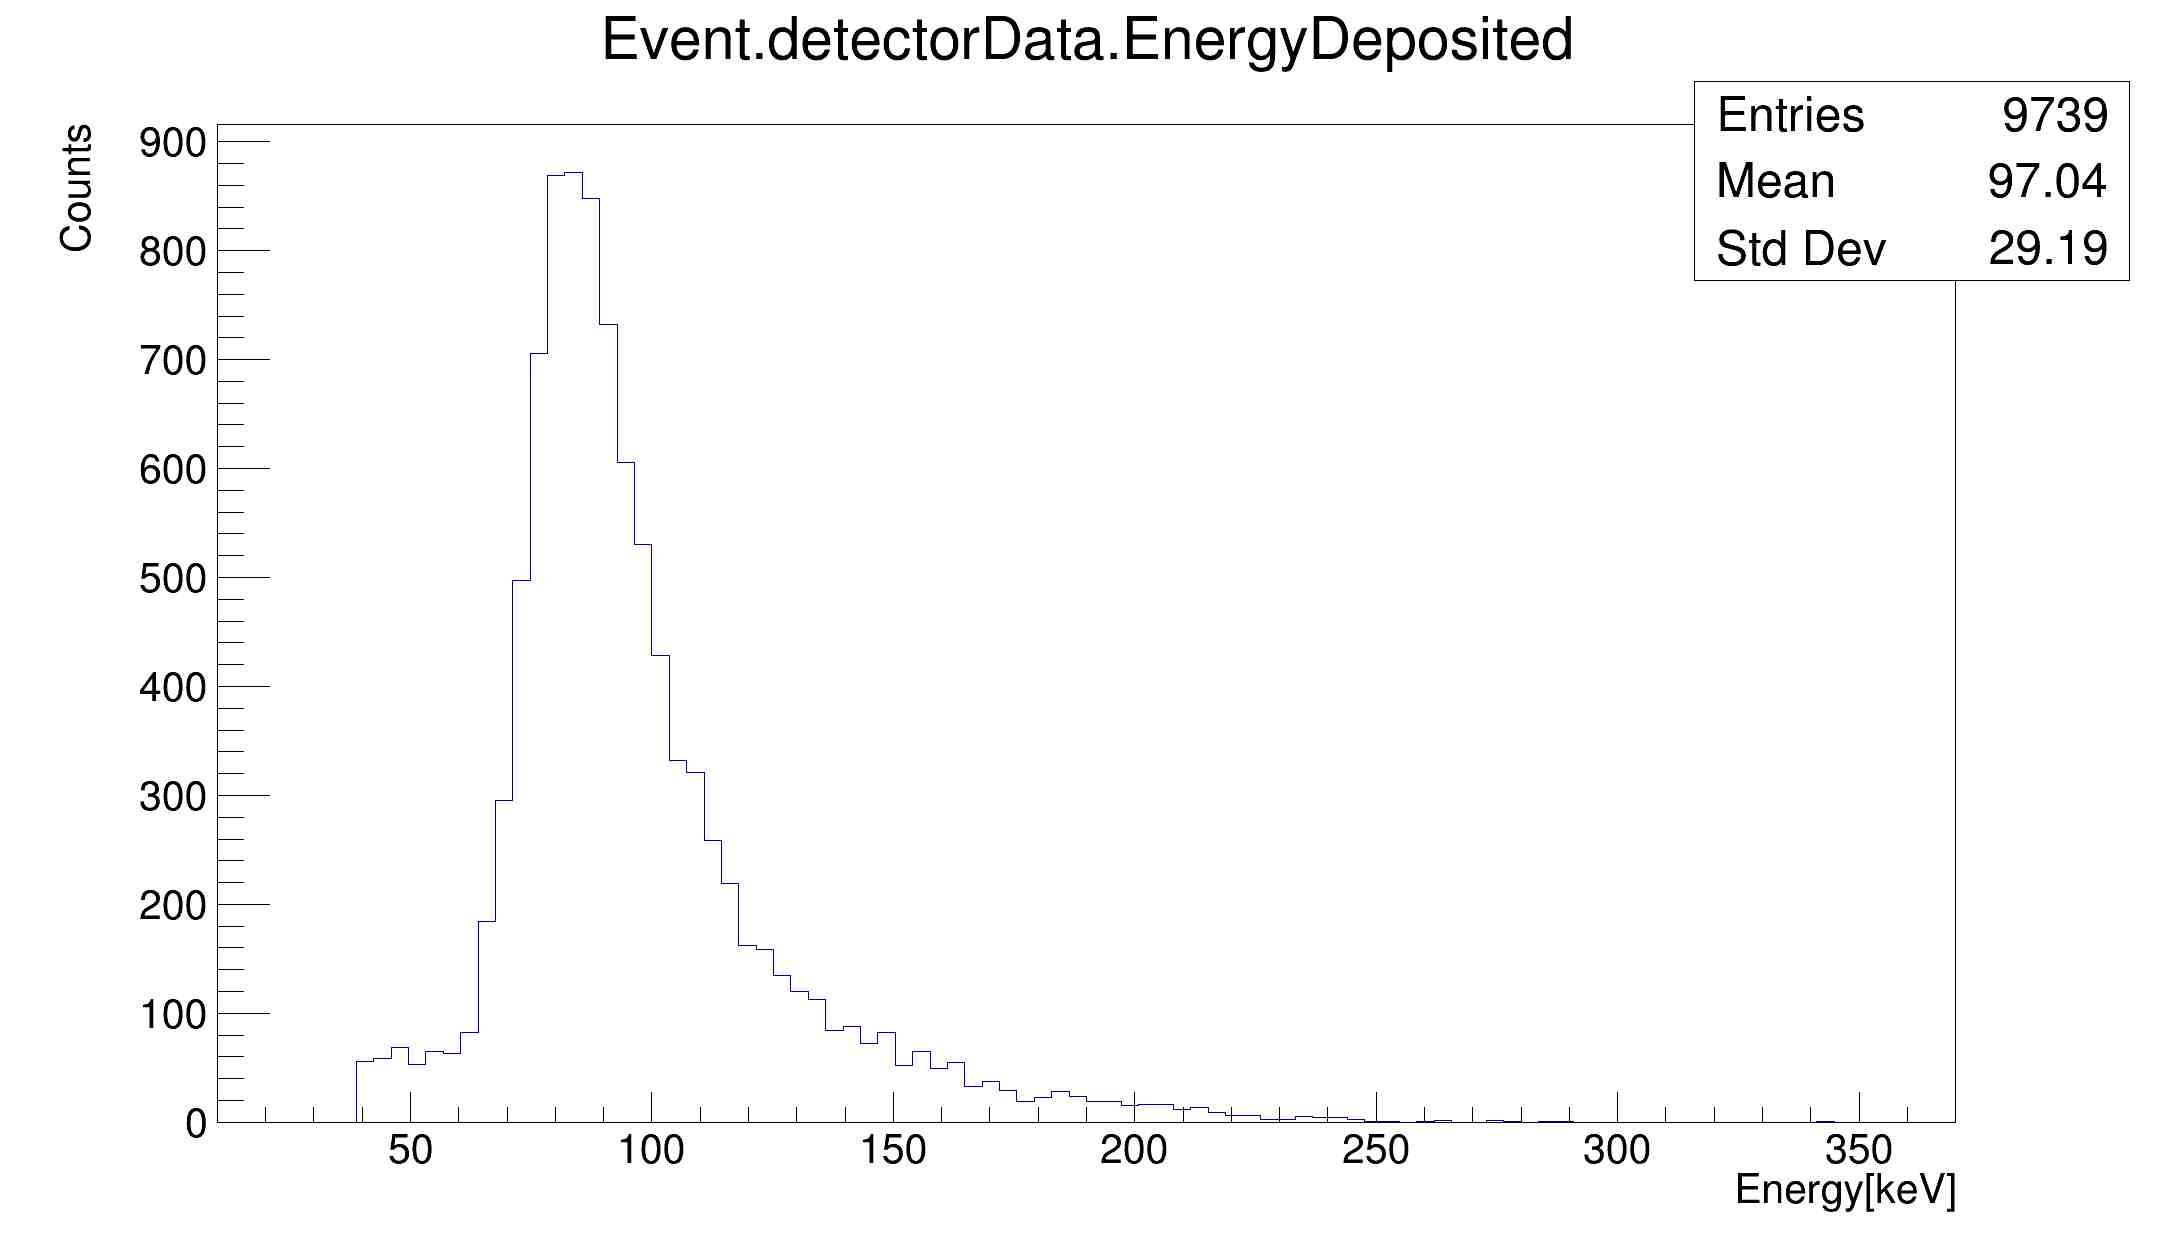
\includegraphics[width=0.52\textwidth]{img/energy.jpg}

       \end{tabular}
       & \begin{tabular}{c}
        \hspace{-8mm}
        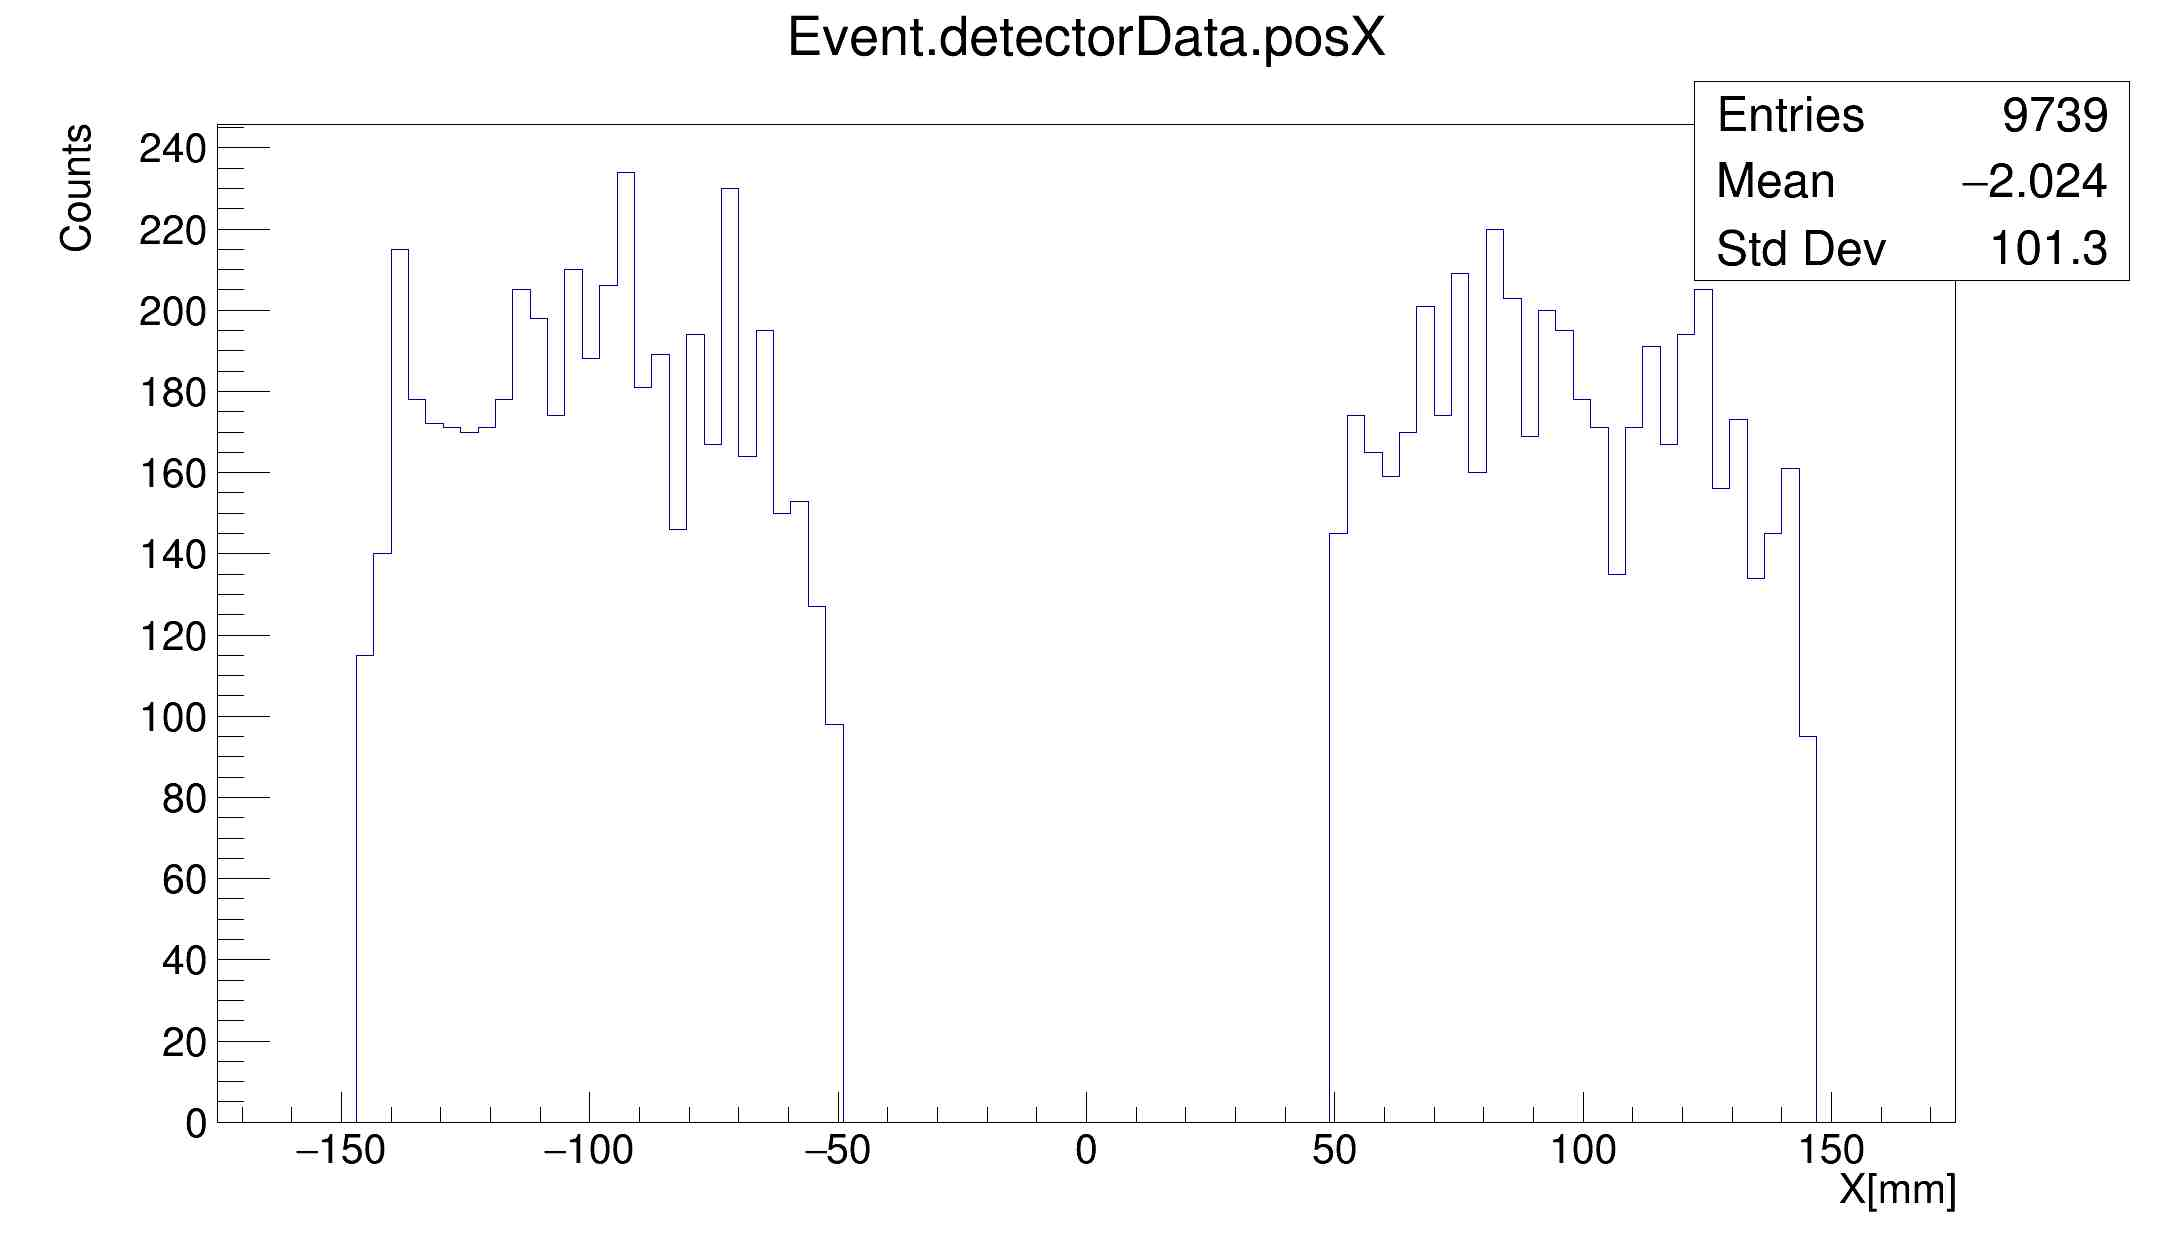
\includegraphics[width=0.52\textwidth]{img/posx.jpg}
            
    \end{tabular}  \\
    \end{tabular}


\end{frame}


\section{Track Reconstruction}

\begin{frame}{Tracking algorithm}
\begin{center}
    Simple toy model: \textbf{Linear fit into the XZ and YZ projections}
\end{center}

$$z=m_x x +x_0$$
$$z=m_y y + y_0$$
\\
\vspace{0.5cm}
\begin{enumerate}
    \item Sort the hits along the z-axis
    \item Compute the initial parameters of the linear function considering only the first and the last point.
    \item Perform the fit exploiting the TGraphError class. (Error bars set to the pitch of strips/pixels divided by $\sqrt{12}$)
\end{enumerate}
\\
    
\end{frame}

\begin{frame}{Reconstructed events}
    
Reconstructed events are saved in an NTuple.
    
\begin{center}
           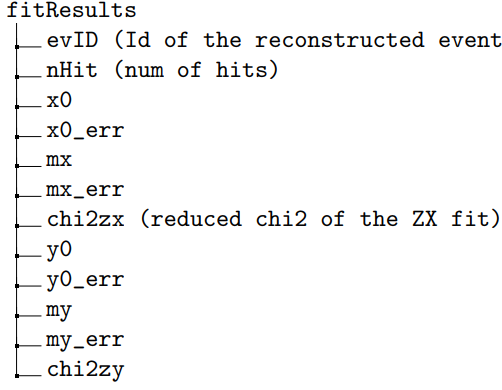
\includegraphics[width=0.5\textwidth]{img/fitres.png}
           \\
           \vspace{0.4cm}
           \\
           \vspace{0.2cm}
           Despite the trigger, there are still events affected by delta rays
\end{center}


    
    
\end{frame}

\begin{frame}[fragile]{Results I}

\begin{figure}[h!]
    \centering
    \subfigure{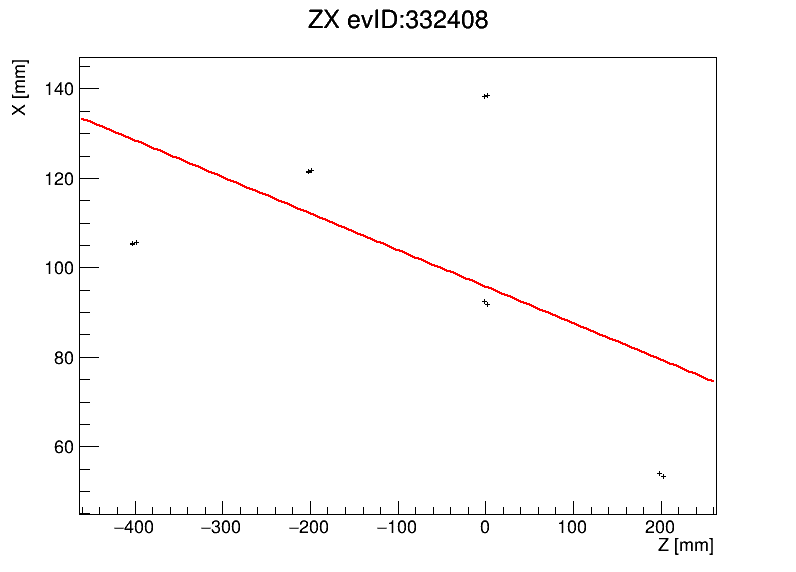
\includegraphics[width=0.48 \textwidth]{img/zx_110870.png}}
    \subfigure{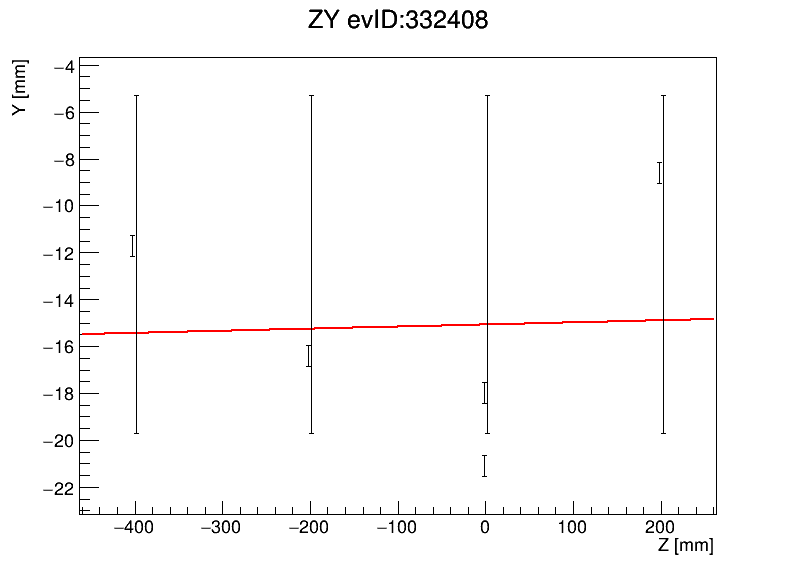
\includegraphics[width=0.48 \textwidth]{img/zy_110870.png}}
    \caption{Event affected by the presence of delta rays' hits}
    \label{fig:bad}
\end{figure}



    
\end{frame}

\begin{frame}{Results II}
\begin{figure}[h!]
    \centering
    \subfigure{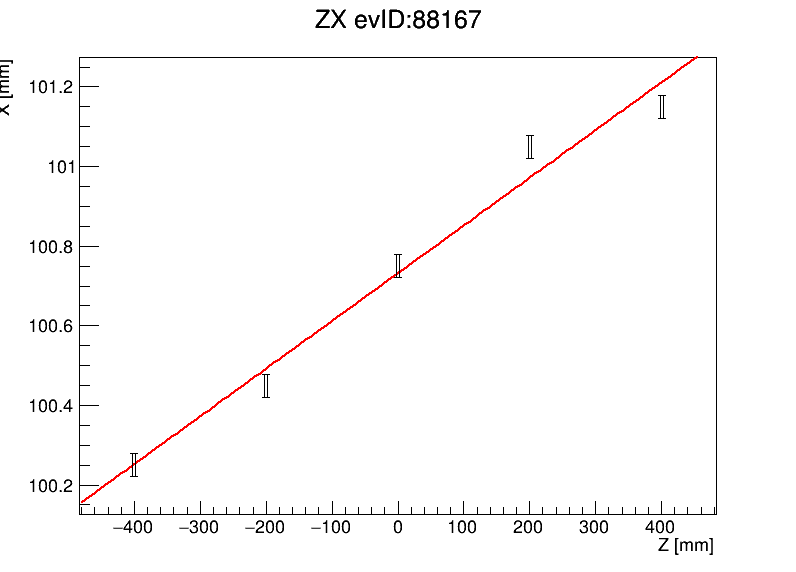
\includegraphics[width=0.48 \textwidth]{img/zx_285208.png}}
    \subfigure{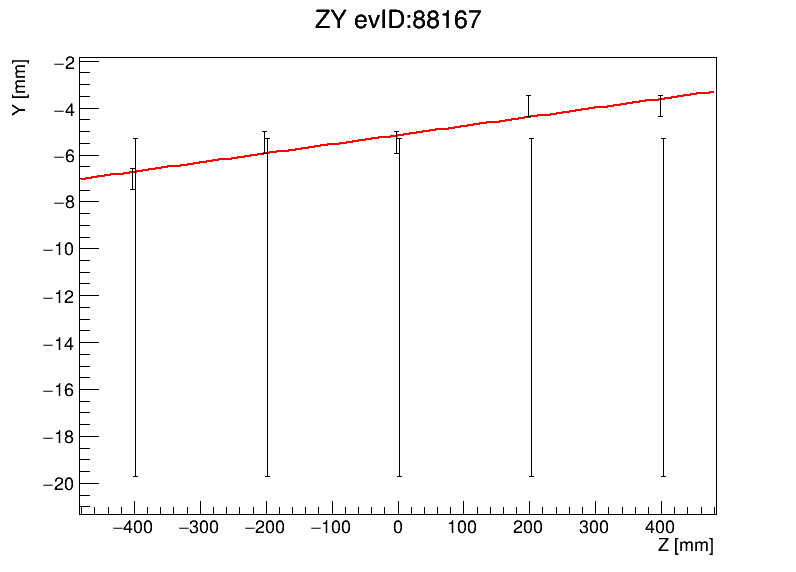
\includegraphics[width=0.48 \textwidth]{img/zy_285208.png}}
    \caption{Well fitted event. Multiple scattering is clearly visible}
    \label{fig:well}
\end{figure}
    
\end{frame}


\begin{frame}{Results III}

\vspace{-0.18cm}
\begin{figure}[h!]
    \centering
    \subfigure{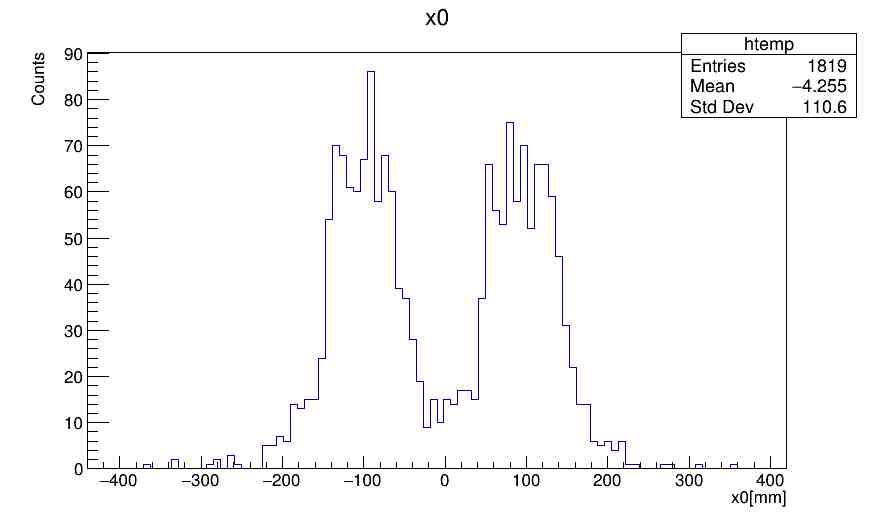
\includegraphics[width=0.54 \textwidth]{img/x0.jpg}}
    \subfigure{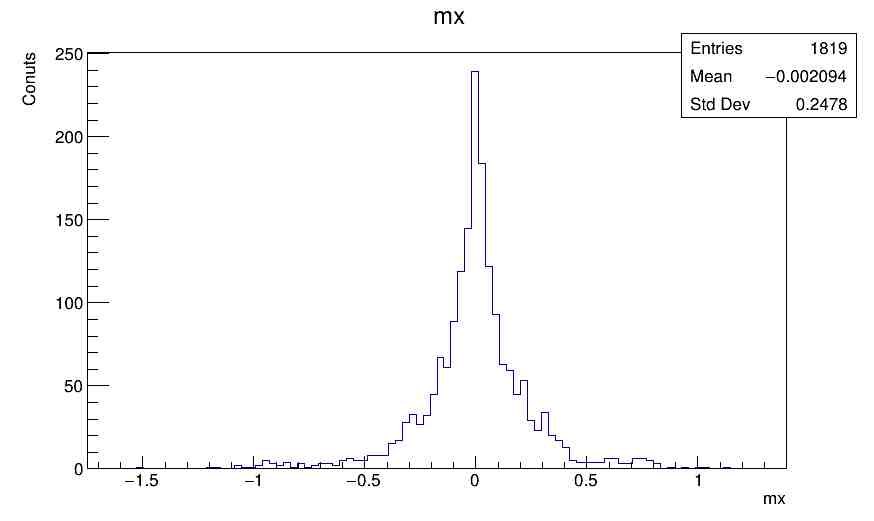
\includegraphics[width=0.54 \textwidth]{img/mx.jpg}}
    \caption{Best fit parameters in the XZ projection}
    \label{fig:well}
\end{figure}



    
\end{frame}



\begin{frame}[allowframebreaks]{References}
 \cite{PS,G4}
  \bibliography{demo}
  \bibliographystyle{abbrv}

\end{frame}

\end{document}
